\chapter{Arquitectura DCI}

  La arquitectura de Datos, Contexto e Interacciones (DCI de sus siglas
  en ingl\'es, Data Context Interaction) es una arquitectura de
  sistemas ideada a lo largo de la carrera de Trygve Reenskaug, el
  creador del patr\'on de presentaci\'on
  Modelo-Vista-Controlador \footnote{MVC, Model View Controller}.

\begin{figure}[!hbtp]
  \centerline{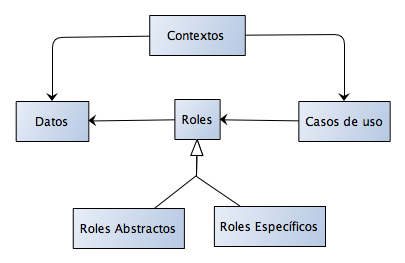
\includegraphics[height=6cm]{dci_overview.png}}
  \caption{Esquema DCI \citep{leanArchitecture} }
\end{figure}

  Ambos, DCI y MVC se orientan hacia la interacci\'on entre personas y
  m\'aquinas, mientras MVC \emph{separa las partes de un programa que
    son responsables de la representaci\'on de la informaci\'on en el
    sistema y las partes que son responsables de la interacci\'on con
    el usuario}, DCI \emph{minimiza cualquier brecha que pueda existir
    entre el modelo mental del programador de su programa y el
    programa que est\'a almacenado y siendo ejecutado en el
    ordenador. En particular, concreta el c\'omo el sistema realiza
    sus operations como una red de objetos en comunicaci\'on}
  \citep{leanArchitecture}.
\\
\\
  Simplificando el concepto de DCI, separa la arquitectura de un
  sistema en la parte de \emph{datos}( el dominio \'o lo que el
  sistema es) y en una \emph{interacci\'on} (lo que el sistema
  hace). La parte de datos se conecta con la parte de interacci\'on a
  trav\'es de una secuencia de eventos denominados el
  \emph{contexto}. La arquitectura puede ser vista como \emph{Datos} e
  \emph{Interacci\'on} din\'amicamente conectados a trav\'es de un
  \emph{Contexto} \citep{leanArchitecture}.

\section{DCI y MVC}
  El objetivo de DCI es separar el c\'odigo que representa el estado
  del sistema del c\'odigo que representa su comportamiento. Esta
  separaci\'on es similar pero diferente a la que realiza MVC.

\begin{figure}[!hbtp]
  \centerline{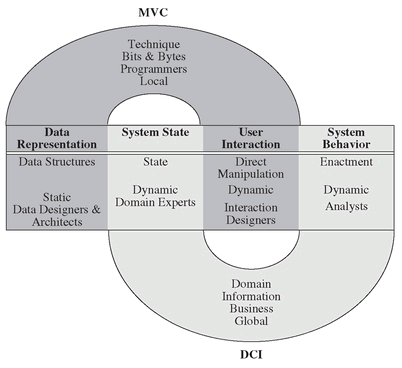
\includegraphics[width=9cm,height=9cm]{dci_arch2.png}}
  \caption{Relaci\'on entre DCI y MVC \citep{leanArchitecture}}
\end{figure}
 
  MVC y DCI est\'an dise\~nados para trabajar juntos como una forma
  de que los programadores razonen sobre el model mental del usuario y
  el c\'omo capturar esos modelos en el c\'odigo.

\section{Ejemplo pr\'actico}
  Tengamos el siguiente escenario en una entidad financiera:
  \begin{quote}

    \emph{Un banco en el cual se realizan los pagos al personal de
    diferentes niveles a trav\'es de la cuenta de su jefe de
    secci\'on, de manera manual a trav\'es de transferencias, requiere
    que este proceso que puede llegar a tomar 2 horas por secci\'on se
    automatice, de forma que el personal pueda enfocar su esfuerzo en
    tareas mas prioritarias.}
  \end{quote}

  En este escenario tenemos que el banco realiza transferencia entre
  cuentas, tales cuentas pueden ser de los gerentes de secci\'on como
  de los empleados, y la tarea a ejecutar es el pago de
  sueldos. Organizando todos estos elementos seg\'un la arquitectura
  DCI tenemos:

  \begin{itemize}
    \item \emph{Objetos del dominio}: Las cuentas bancarias, simples
      objetos con s\'olo los atributos y comportamientos b\'asicos de
      una cuenta.

    \item \emph{Roles}: Al ser las cuentas bancarias entidades
      b\'asicas de negocio, los roles definen el comportamiento de
      estos objetos para una o varias responsabilidades
      espec\'ificas. Para este caso, tenemos que las cuentas de
      empleados reciben el dinero, mientras que las cuentas de los
      gerentes transfieren dinero.

    \item \emph{Contexto}: El contexto viene a ser el evento en s\'i,
      el deposito de sueldos, lo que hace el contexto es crear cuentas
      y agregarles comportamiento de forma din\'amica, siendo los
      gerentes aquellos que depositan dinero a las cuentas
      empleado. No es posible que las cuentas empleados puedan
      realizar otras operaciones porque no tienen esas capacidades en
      este contexto, asimismo para las cuentas de gerentes, solamente
      tienen \emph{inyectado} el comportamiento necesario para
      realizar el dep\'osito de sueldos. De esta forma el dominio y la
      sem\'antica de la operaci\'on se reduce exactamente a lo que el
      usuario realmente quiere hacer.

  \end{itemize}
